\documentclass[dvipdfmx]{jsarticle}

\usepackage[utf8]{inputenc}
\usepackage{graphicx}
\usepackage{float}
\usepackage{amsmath}
\begin{document}
\title{人工知能 課題番号09  \\Wuの定理の実装}
\author{電気電子工学科 03-180500\\ 平井雄太}
\date{2018年11月5日}
\maketitle

\section{プログラムの使い方}
本課題では、Wuの定理に基づく幾何の自動定理証明システムを実装した。プログラムの簡単な使い方と注意すべき点を以下に記す。

\subsection{必要な実行環境}
python3

sympy(python用のライブラリ)

以上がインストールされている必要がある。

\subsection{基本的な使い方}
本プログラムは以下のように使用する。まず、単にプログラムを実行したいだけであれば、
\begin{quote}
\$python3 Wu.py 
\end{quote}
と入力する。すると仮定と結論を入力するように促されるので、それらを入力し、最後に空行を入力するWuの手続きを実行する。この時、数式の入力はpythonの入力形式に則るものとする。例えば,$x^2$は$x**2$と入力する。ここで、\underline{変数はアルファベット大文字小文字の1文字のみが許される。}また、変数を使用する際には、\underline{アルファベットの小さい順から使用しなくてはならない}ので注意が必要である。例えば、変数に"x1"などは使えないし、変数として(a, b, d)などを用いてはならない。
\subsection{従属変数の選定}
デフォルトでは、従属変数はアルファベット順に小さい方から仮定の数の分だけ選んだものが使用される。例えば仮定の数が全部で7個であれば,従属変数として
\begin{quote}
(a, b, c, d, e, f, g)
\end{quote}
が従属変数として使用される。個別に従属変数を設定するには以下のようにする。例えば
\begin{quote}
(b, c, f, g, j, i, h)
\end{quote}
を従属変数として用いるには
\begin{quote}
\$python3 Wu.py --vars b,c,f,g,j,i,h
\end{quote}
とすればいい。ただし\underline{変数間に空白を含めてはいけない}。また、\underline{変数の数は仮定の数と同じにする必要があり}、\underline{同じ変数を重複させて含めてはいけない}。

\subsection{外部ファイルからの読み取り}
外部ファイルから仮定と結論を読み取ることが可能である。最初に仮定を、最後の1行に結論を記入しておく。例えば, Pythagollas.txtに
\begin{quote}
a*c+b*d

a**2+b**2+c**2+d**2-(a-c)**2-(b-d)**2
\end{quote}
という式が格納されていたとする。この時、プログラムは
\begin{quote}
\$python3 Wu.py --file Pythagollas.txt 
\end{quote}
と入力することにより実行される。

\subsection{その他}
\begin{quote}

\$python3 Wu.py --latex
\end{quote}
とすることで,数式を{\LaTeX}形式で出力することが可能である。
また、
\begin{quote}
\$python3 Wu.py --help
\end{quote}
と入力することで簡単な説明を見ることができる。
\clearpage
\section{本プログラムを用いたいくつかの定理の証明}
本プログラムを用いていくつかの定理の自動証明を行なった。なお、これらの定理の仮定と結論の式は全てテキストファイルとして添付してある。
    \subsection{ピタゴラスの定理}
        \begin{figure}[H]
            \centering
            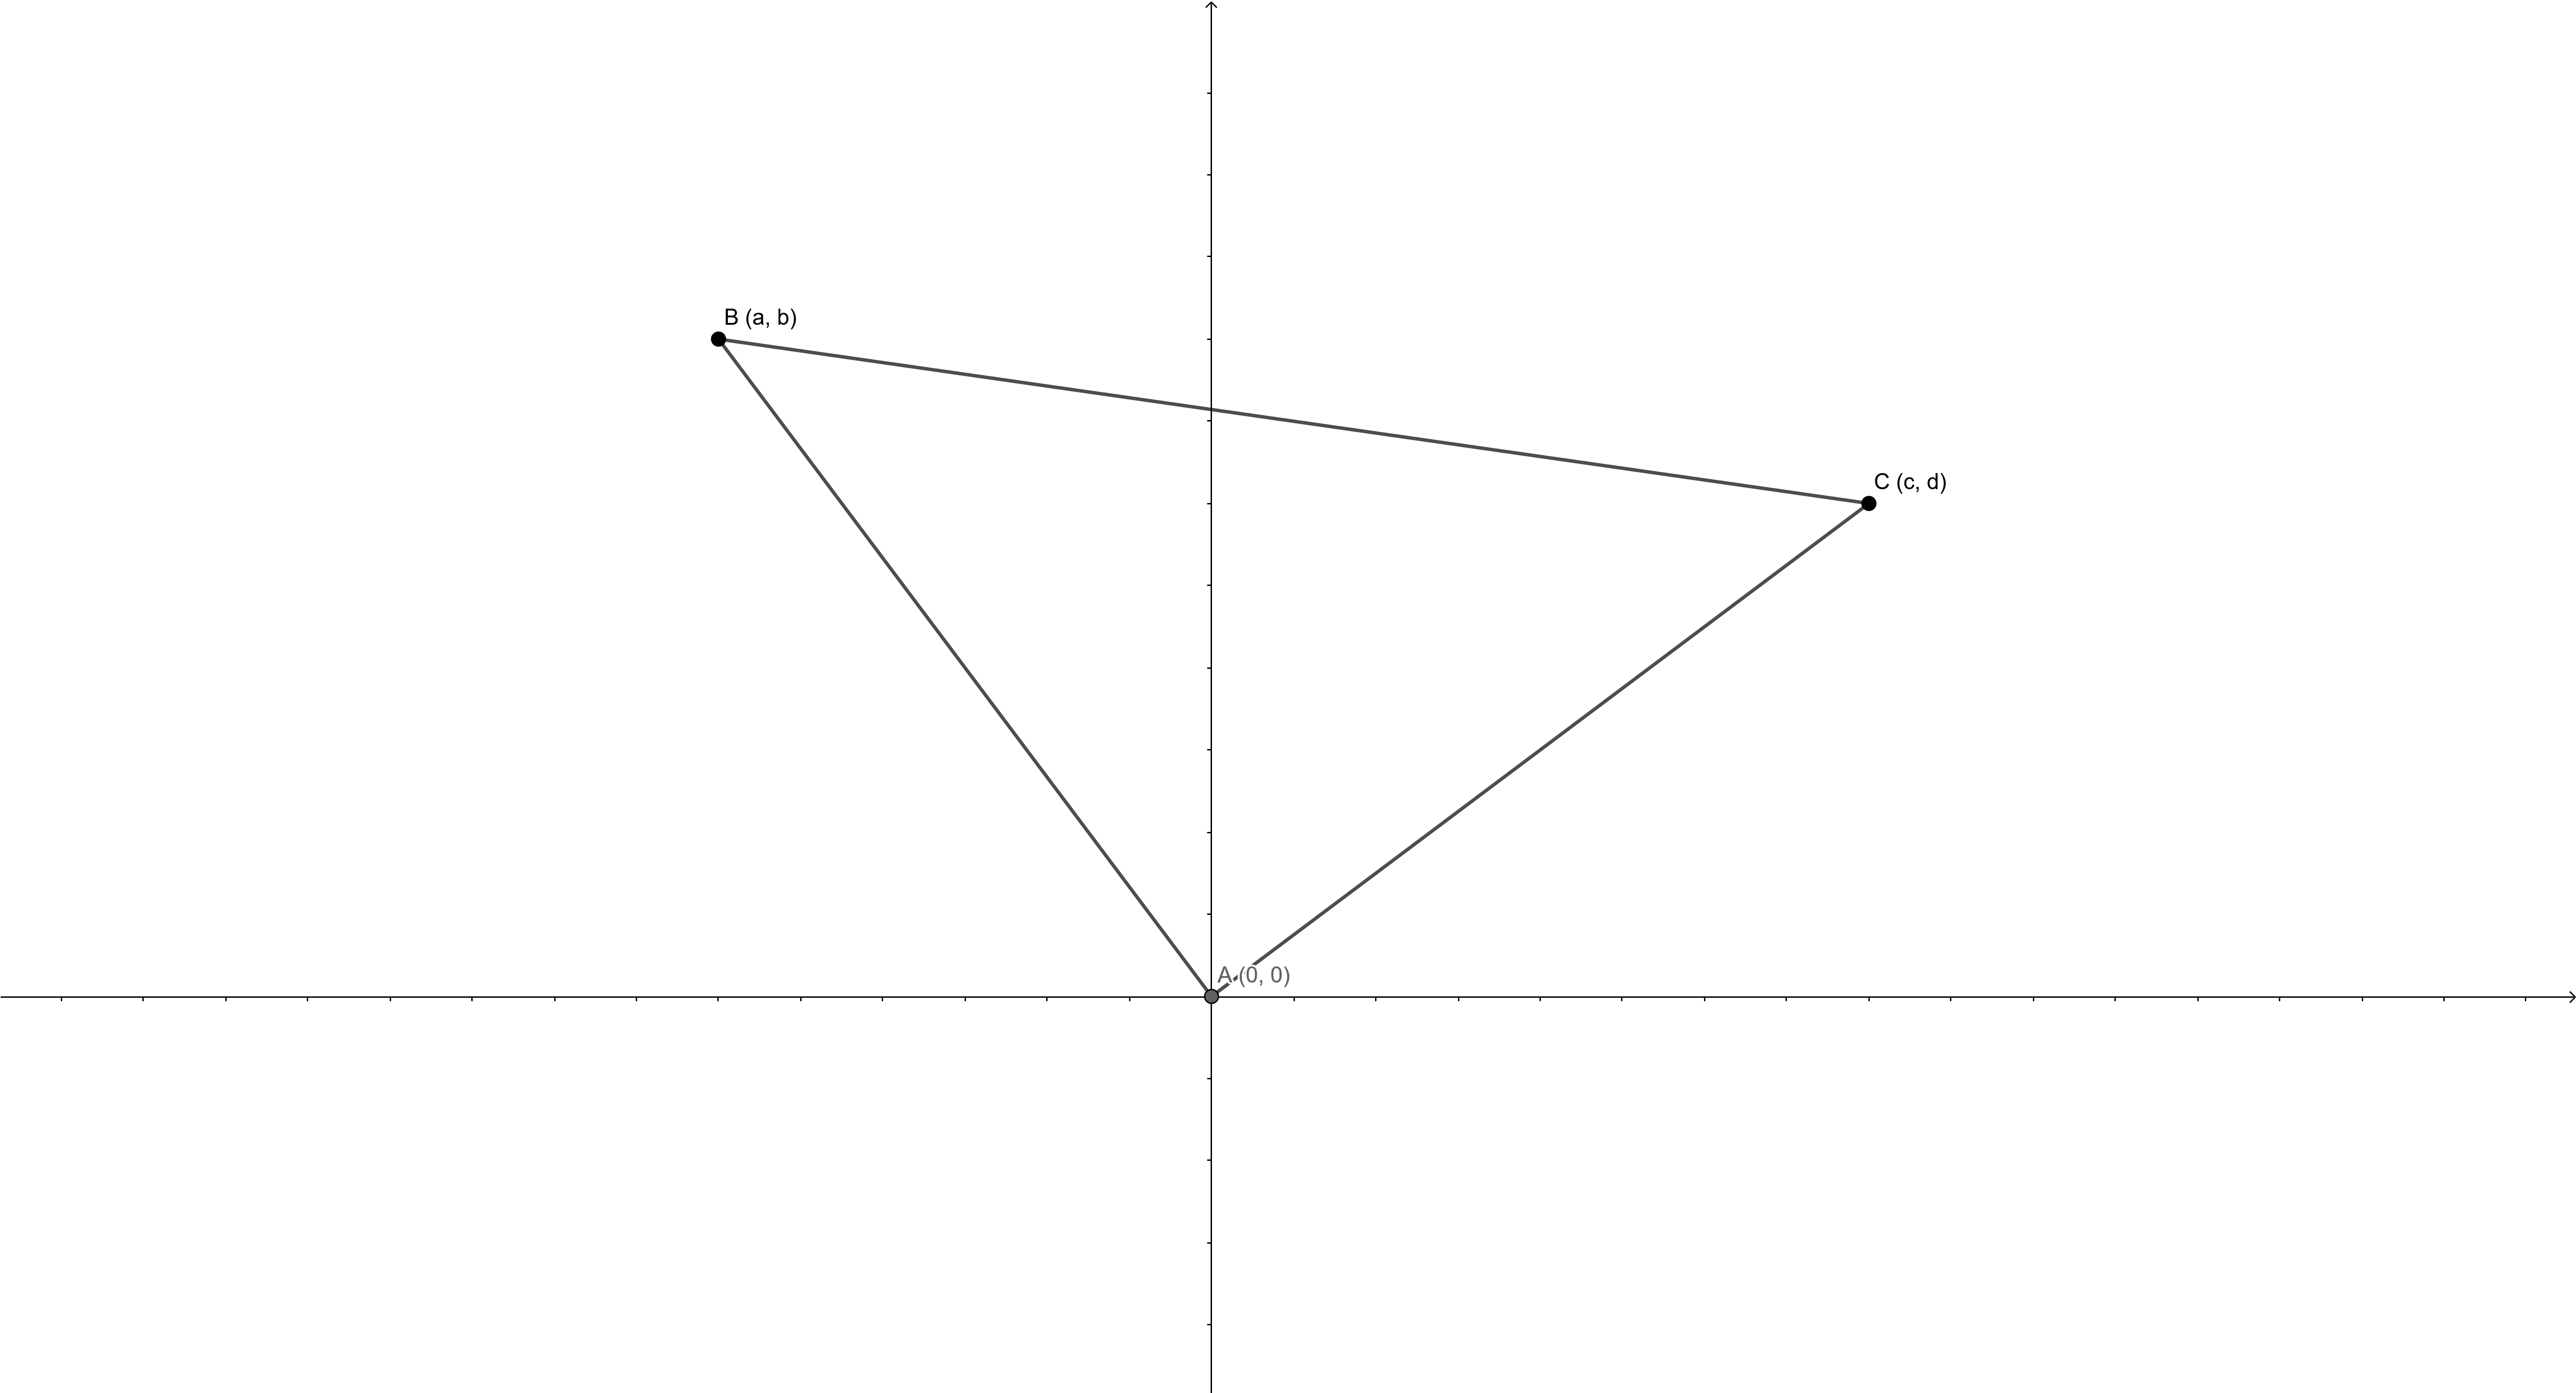
\includegraphics[width=10cm]{Pythagoras.png}
            \caption{ピタゴラスの定理}
            \label{fig:Pythagoras}      
        \end{figure}

        
        \begin{table}[H]
            \label{table:PythagorasAssumption}
            \centering
            \caption{ピタゴラスの定理の仮定と結論の式}
            \begin{tabular}{cc}
                仮定 と 結論 & 意味\\
                \hline \hline
                $Hyp_{1} = a c + b d$ & ABとACは垂直\\
                $Conc =a^{2} + b^{2} + c^{2} + d^{2} - \left(a - c\right)^{2} - \left(b - d\right)^{2}$ & $BC^2=AB^2+AC^2$ \\
            \end{tabular}
        \end{table}

        \begin{figure}[H]
            \centering
            \label{fig:PythagorasTri}
            \fbox{$
                \begin{aligned}
                    Tri_{1}(a) = a c + b d
                \end{aligned}
            $}
            \caption{ピタゴラスの定理の三角形式}
        \end{figure}

        \begin{figure}[H]
            \centering
            \label{fig:PythagorasWu}
            \fbox{$
                \begin{aligned}
                    Rem_{0} &= a^{2} + b^{2} + c^{2} + d^{2} - \left(a - c\right)^{2} - \left(b - d\right)^{2}\\
                    Rem_{1} &= 0\\
                    Subsidaries &= c
                \end{aligned}$}
            \caption{ピタゴラスの定理のWuの手続きの実行過程}            
        \end{figure}
    \clearpage
    \subsection{アポロニウスの円}
    \begin{figure}[H]
        \centering
        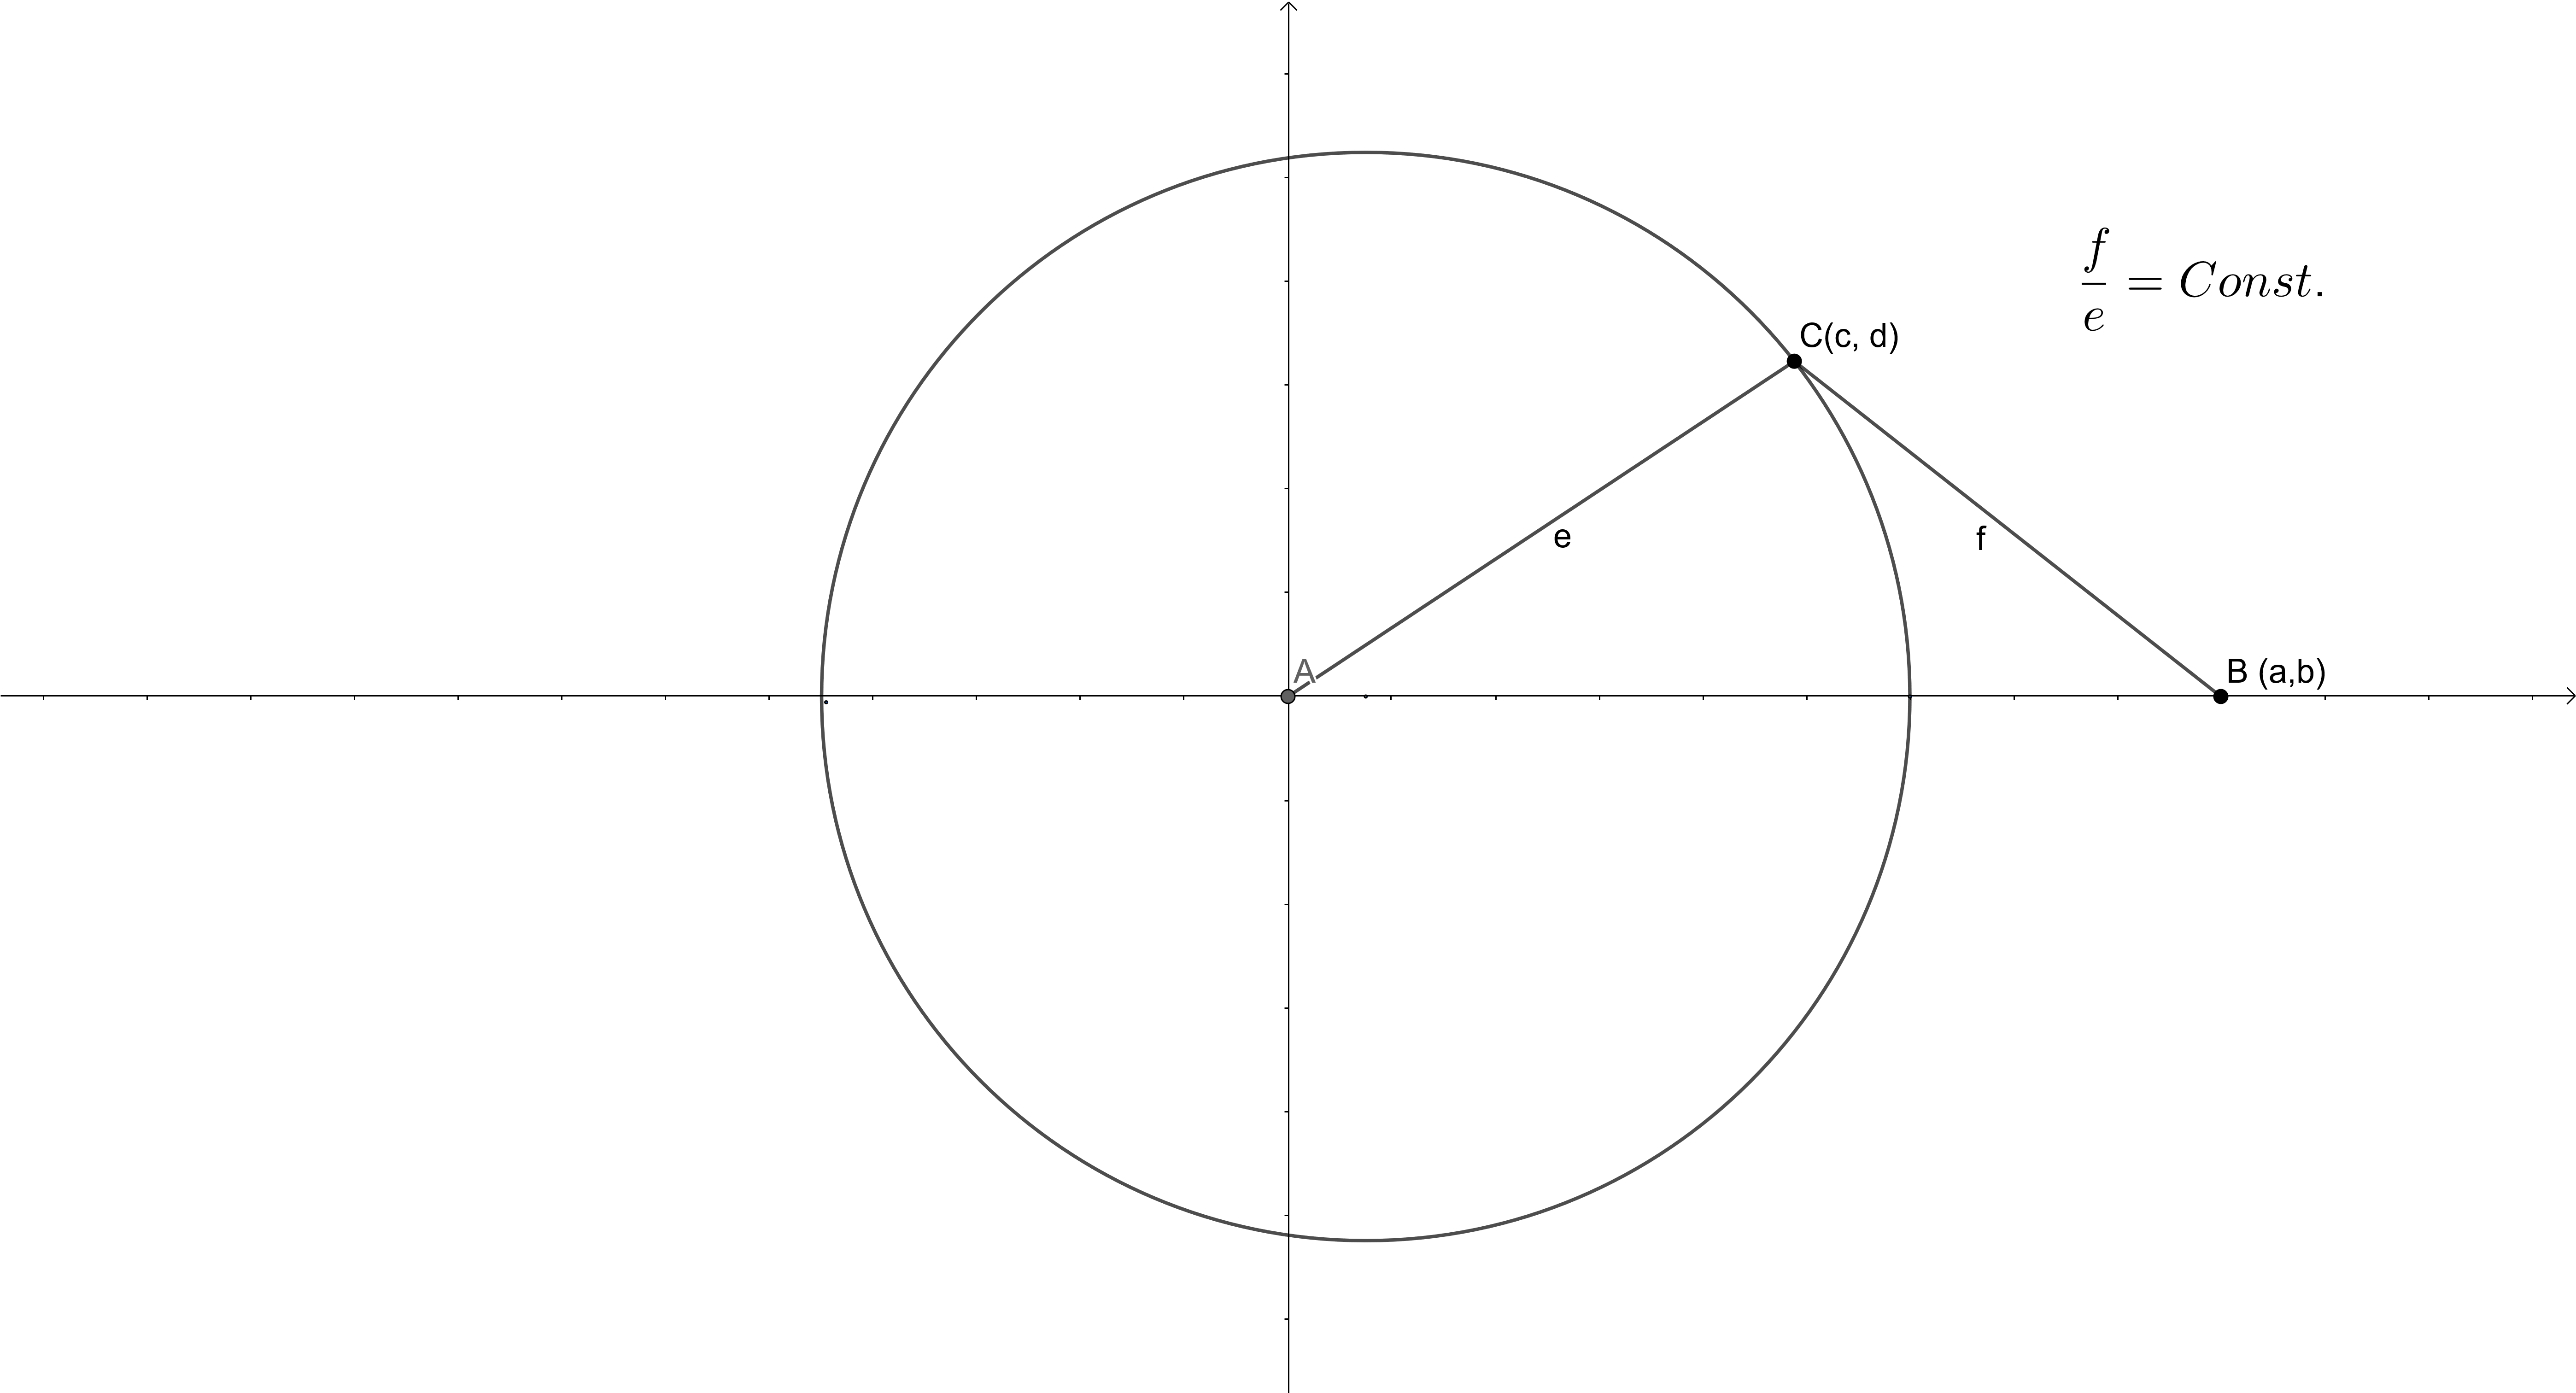
\includegraphics[width=10cm]{Appollonius.png}
        \caption{アポロニウスの円}
        \label{figure:Appollonius}
    \end{figure}
    \begin{table}[H]
        \caption{アポロニウスの円の仮定と結論}
        \centering
        \begin{tabular}{cc}
            仮定と結論 & 意味 \\
            \hline \hline
            $Hyp_{1} = - b^{2} + c^{2} + f^{2}$ & fは辺ACの長さ \\
            $Hyp_{2} = - c^{2} + g^{2} - \left(a - b\right)^{2}$ & gは辺BCの長さ \\
            $Hyp_{3} = - e g + f$ & fとgの比は一定 \\
            $Conc =\left(- \frac{a f}{f + g} + f\right) \left(- \frac{a g}{f + g} + g\right)$ & 円の半径は$\frac{a f}{f + g}$あるいは$\frac{a g}{f + g}$ \\
        \end{tabular}
    \end{table}
    \begin{figure}[H]
        \centering
        \fbox{$
            \begin{aligned}
                Tri_{1}(a, b, c) &= - b^{2} + c^{2} + f^{2} \\
                Tri_{2}(a, b) &= - a^{2} + 2 a b - 2 b^{2} + f^{2} + g^{2} \\
                Tri_{3}(a) &= - e g + f \\
            \end{aligned}$}
        \caption{アポロニウスの円の三角形式}
    \end{figure}
    \begin{figure}[H]
        \centering
        \fbox{$
            \begin{aligned}
                Rem_{0} &= \left(- \frac{a f}{f + g} + f\right) \left(- \frac{a g}{f + g} + g\right) \\
                Rem_{1} &= \frac{1}{f^{2} + 2 f g + g^{2}} \left(a^{2} f g - 2 a f^{2} g - 2 a f g^{2} + f^{3} g + 2 f^{2} g^{2} + f g^{3}\right)\\
                Rem_{2} &= \frac{1}{f^{2} + 2 f g + g^{2}} \left(a^{2} f g - 2 a f^{2} g - 2 a f g^{2} + f^{3} g + 2 f^{2} g^{2} + f g^{3}\right)\\
                Rem_{3} &= 0\\
                Subsidaries &= 2 e g - 2 f\\
            \end{aligned}
        $}
        \caption{アポロニウスの円のWuの手続きの実行過程}
    \end{figure}
    \clearpage
    \subsection{ナポレオンの定理}
    \begin{figure}[H]
        \centering
        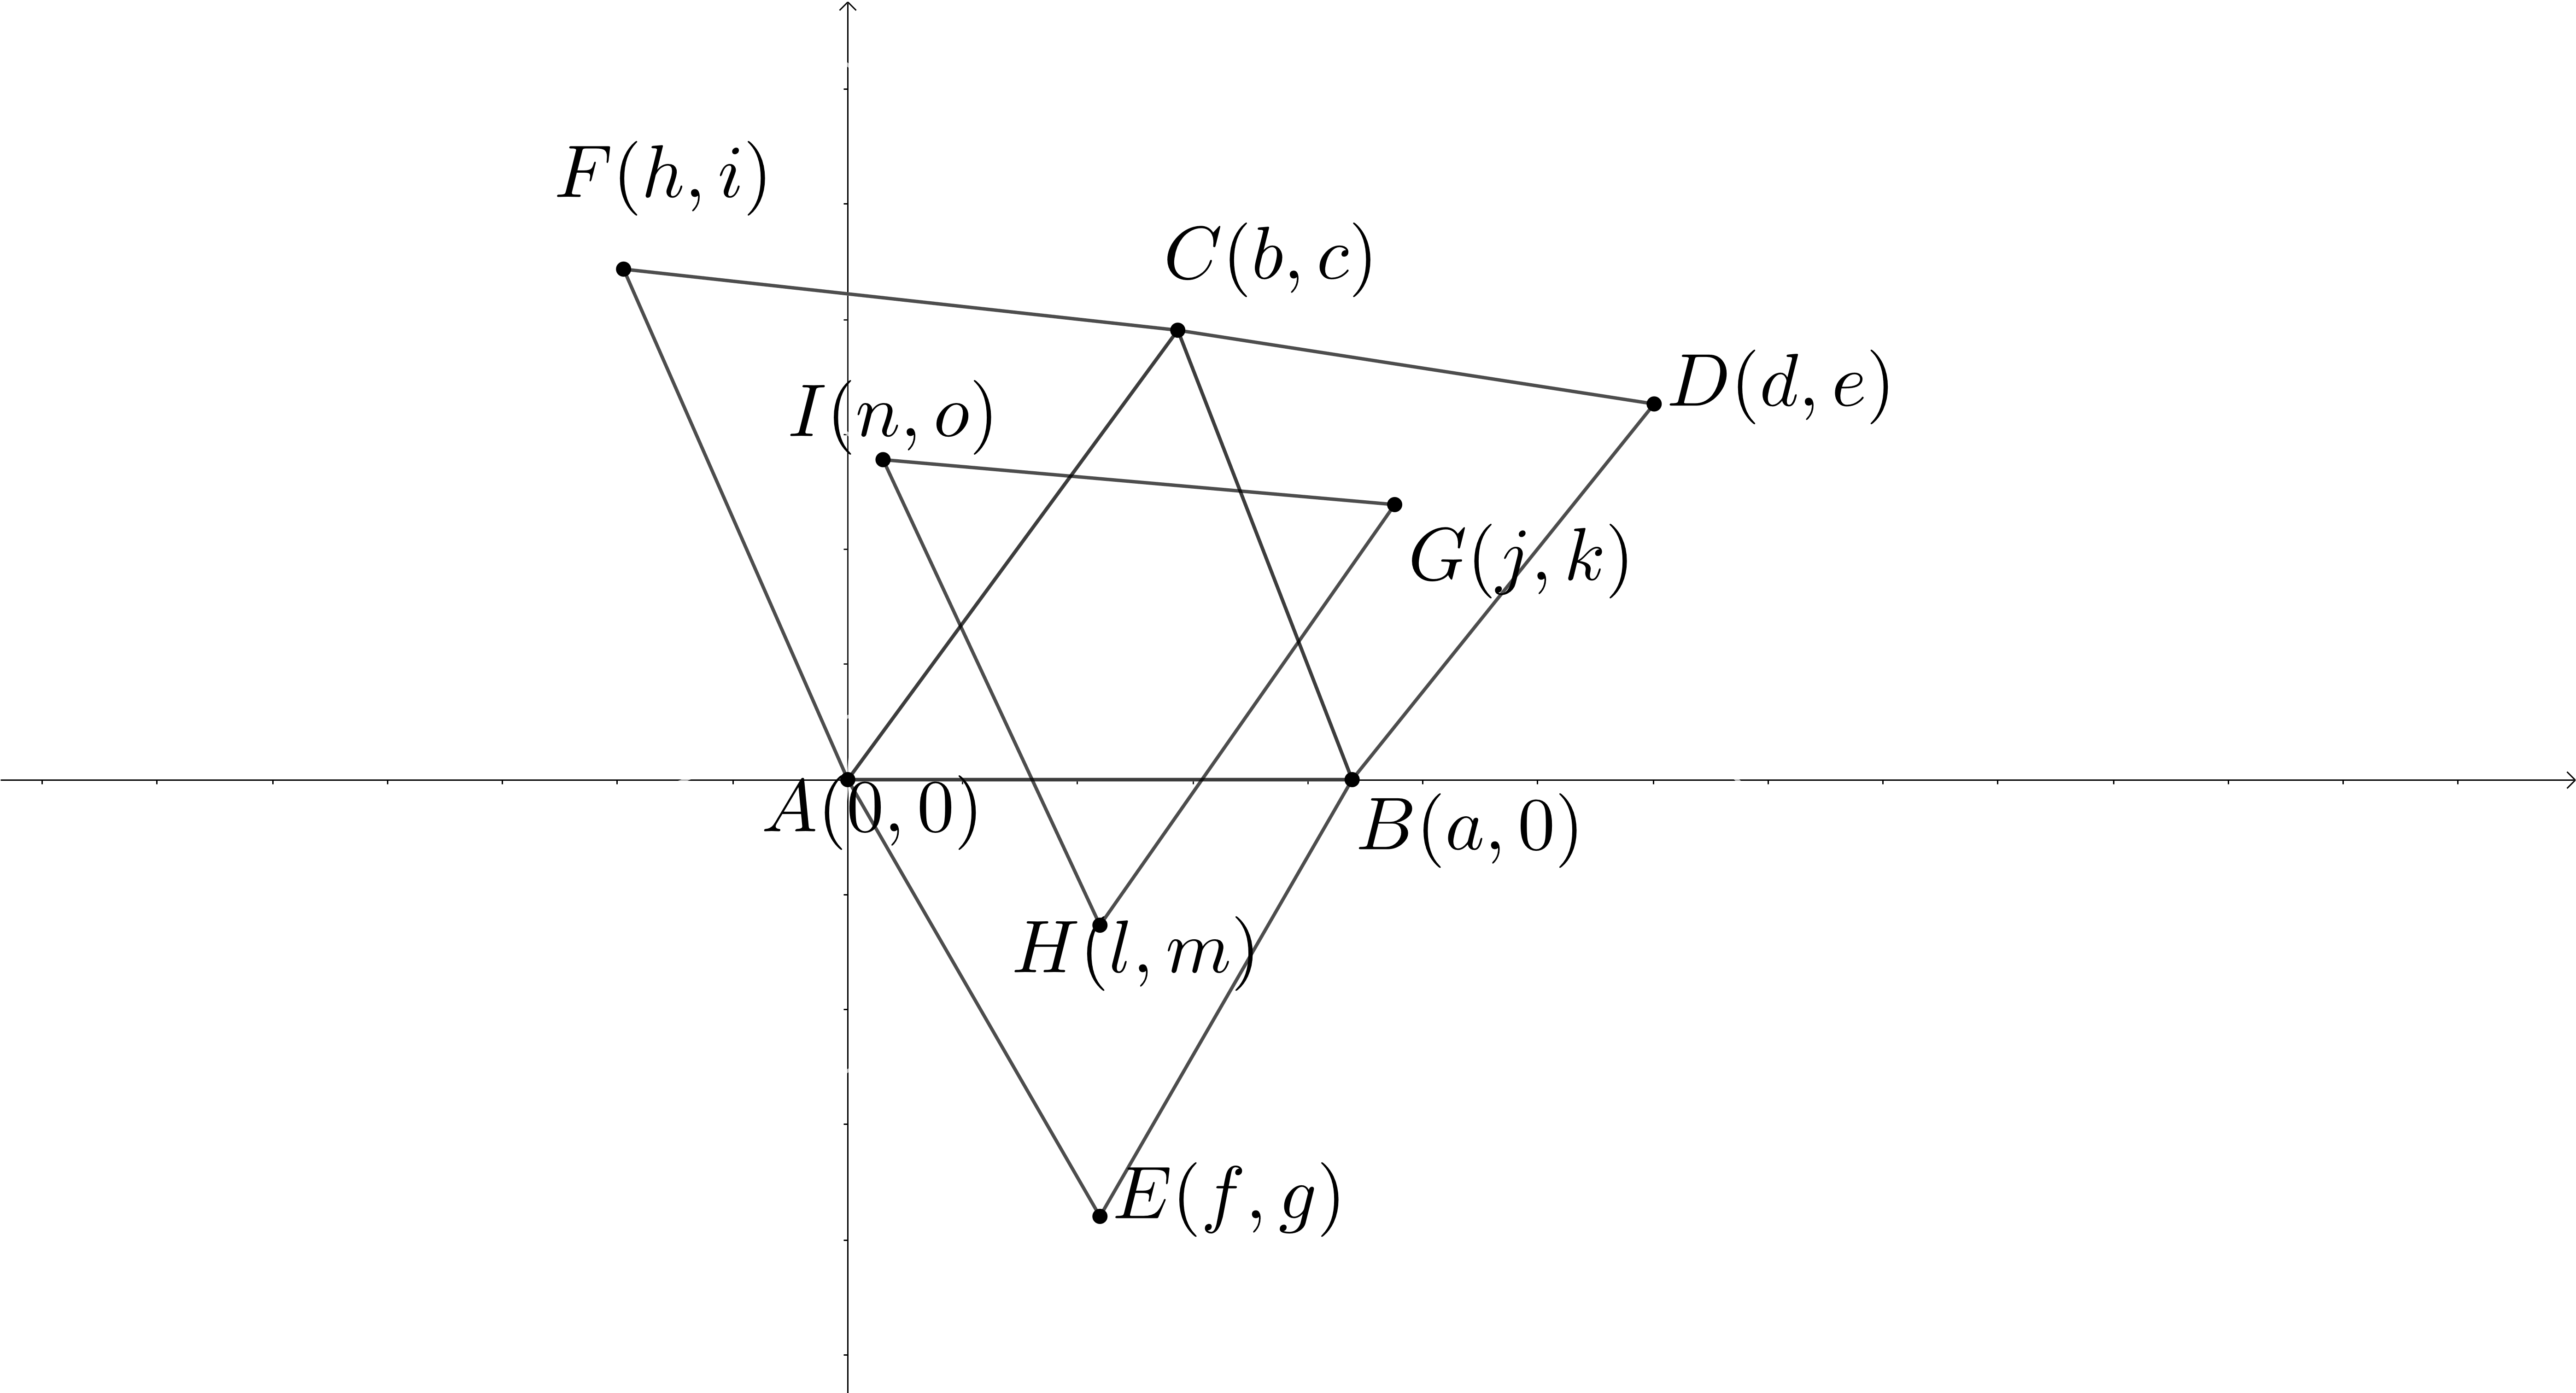
\includegraphics[width=10cm]{Napoleon.png}
        \caption{ナポレオンの定理}
    \end{figure}
    \begin{table}[H]
        \centering
        \caption{ナポレオンの定理の結論と仮説}
        \begin{tabular}{cc}
            結論と仮定 & 意味 \\
            \hline \hline
            $Hyp_{1} = - b^{2} - c^{2} + \left(b - h\right)^{2} + \left(c - i\right)^{2}$ & $AC=FC$\\
            $Hyp_{2} = - b^{2} - c^{2} + h^{2} + i^{2}$& $AC=AF$\\
            $Hyp_{3} = - c^{2} - \left(a - b\right)^{2} + \left(b - d\right)^{2} + \left(c - e\right)^{2}$&$BC=CD$\\
            $Hyp_{4} = - c^{2} + e^{2} - \left(a - b\right)^{2} + \left(a - d\right)^{2}$&$BC=BD$\\
            $Hyp_{5} = - a^{2} + f^{2} + g^{2}$&$AB=AE$\\
            $Hyp_{6} = - a^{2} + g^{2} + \left(- a + f\right)^{2}$&$AB=BE$\\
            $Hyp_{7} = - b - h + 3 n$&$Iは\triangle{ACF}の重心$\\
            $Hyp_{8} = - c - i + 3 o$&$Iは\triangle{ACF}の重心$\\
            $Hyp_{9} = - a - b - d + 3 j$&$Gは\triangle{BCD}の重心$\\
            $Hyp_{10} = - c - e + 3 k$&$Gは\triangle{BCD}の重心$\\
            $Hyp_{11} = - a - f + 3 l$&$Hは\triangle{ABE}の重心$\\
            $Hyp_{12} = - g + 3 m$&$Hは\triangle{ABE}の重心$\\
            $Hyp_{13} = \frac{\sqrt{3} a}{2} + m$&$Iはtriangle{ACF}の外側という条件のために必要$\\
            $Hyp_{14} = - \frac{c}{2} + e - \frac{\sqrt{3}}{6} \left(a - b\right)$&$Gはtriangle{BCD}の外側という条件のために必要$\\
            $Hyp_{15} = - \frac{b}{2} + \frac{\sqrt{3} c}{2} + h$&$Hはtriangle{ABE}の外側という条件のために必要$\\
            $Conc =- \left(- j + l\right)^{2} - \left(- k + m\right)^{2} + \left(- l + n\right)^{2} + \left(- m + o\right)^{2}$&$HI=HG(triangle{GHI}は正三角形)$\\
        \end{tabular}
    \end{table}
    \begin{figure}[H]
        \centering
        \fbox{$
            \begin{small}
            \begin{aligned}
            Tri_{1}(a, b, c, d, e, f, g, h, i, j, k, l, m, n, o) &= - c - i + 3 o \\
            Tri_{2}(a, b, c, d, e, f, g, h, i, j, k, l, m, n) &= - b - h + 3 n \\
            Tri_{3}(a, b, c, d, e, f, g, h, i, j, k, l, m) &= - g + 3 m \\
            Tri_{4}(a, b, c, d, e, f, g, h, i, j, k, l) &= - a - f + 3 l \\
            Tri_{5}(a, b, c, d, e, f, g, h, i, j, k) &= - c - e + 3 k \\
            Tri_{6}(a, b, c, d, e, f, g, h, i, j) &= - a - b - d + 3 j \\
            Tri_{7}(a, b, c, d, e, f, g, h, i) &= - b^{2} + 2 b h - c^{2} + 2 c i \\
            Tri_{8}(a, b, c, d, e, f, g, h) &= - \frac{b}{2} + \frac{\sqrt{3} c}{2} + h \\
            Tri_{9}(a, b, c, d, e, f, g) &= \frac{3 a}{2} \sqrt{3} + g \\
            Tri_{10}(a, b, c, d, e, f) &= a^{2} - 2 a f \\
            Tri_{11}(a, b, c, d, e) &= - \frac{c}{2} + e - \frac{\sqrt{3}}{6} \left(a - b\right) \\
            Tri_{12}(a, b, c, d) &= a^{2} + \frac{a c}{3} \sqrt{3} - b^{2} - \frac{b c}{3} \sqrt{3}
            \\ &\quad + d \left(- 2 a + 2 b\right) \\
            Tri_{13}(a, b, c) &= - \frac{8 a^{4}}{3} + \frac{32 b}{3} a^{3} - 16 a^{2} b^{2} - \frac{8 a^{2}}{3} c^{2} 
            \\ &\quad + \frac{32 a}{3} b^{3} + \frac{16 a}{3} b c^{2} - \frac{8 b^{4}}{3} - \frac{8 b^{2}}{3} c^{2}\\
            Tri_{14}(a, b) &= 24 a^{4}\\
            Tri_{15}(a) &= 0\\
        \end{aligned}
        \end{small}
        $}
        \caption{ナポレオンの定理の三角形式}
    \end{figure}
    \begin{figure}[H]
        \centering
        \fbox{$
            \begin{aligned}
                Rem_{0} &= - (- j + l)^{2} - (- k + m)^{2} + 
                \\ &\quad (- l + n)^{2} + (- m + o)^{2}\\
                Rem_{1} &= c^{2} + 2 c i - 6 c m + i^{2} - 6 i m - 9 j^{2} 
                \\ &\quad + 18 j l - 9 k^{2} + 18 k m - 18 l n + 9 n^{2} \\
                Rem_{2} &= 9 b^{2} + 18 b h - 54 b l + 9 c^{2} + 18 c i 
                \\ &\quad - 54 c m + 9 h^{2} - 54 h l + 9 i^{2} - 54 i m 
                \\ &\quad - 81 j^{2} + 162 j l - 81 k^{2} + 162 k m\\
                Rem_{3} &= 27 b^{2} + 54 b h - 162 b l + 27 c^{2} 
                \\ &\quad - 54 c g + 54 c i - 54 g i + 162 g k 
                \\ &\quad + 27 h^{2} - 162 h l + 27 i^{2} - 243 j^{2} 
                \\ &\quad + 486 j l - 243 k^{2}\\
                Rem_{4} &= - 162 a b - 162 a h + 486 a j + 81 b^{2} 
                \\ &\quad - 162 b f + 162 b h + 81 c^{2} - 162 c g 
                \\ &\quad + 162 c i - 162 f h + 486 f j - 162 g i 
                \\ &\quad + 486 g k + 81 h^{2} + 81 i^{2} - 729 j^{2} - 729 k^{2}\\
                Rem_{5} &= - 1458 a b - 1458 a h + 4374 a j + 729 b^{2} 
                \\ &\quad - 1458 b f + 1458 b h - 1458 c e + 1458 c i - 729 e^{2} 
                \\ &\quad + 1458 e g - 1458 f h + 4374 f j - 1458 g i + 729 h^{2} + 729 i^{2} - 6561 j^{2}\\
                Rem_{6} &= 6561 a^{2} - 13122 a b + 13122 a f - 13122 a h - 13122 b d 
                \\ &\quad + 13122 b h - 13122 c e + 13122 c i - 6561 d^{2} 
                \\ &\quad + 13122 d f - 6561e^{2} + 13122 e g - 13122 f h 
                \\ &\quad - 13122 g i + 6561 h^{2} + 6561 i^{2}\\
                Rem_{7} &= 26244 a^{2} c^{2} - 52488 a b c^{2} 
                \\ &\quad + 52488 a c^{2} f - 52488 a c^{2} h 
                \\ &\quad + 6561 b^{4} - 26244 b^{3} h + 39366 b^{2} c^{2} 
                \\ &\quad - 26244 b^{2} c g + 26244 b^{2} h^{2} 
                \\ &\quad - 52488 b c^{2} d - 26244 b c^{2} h + 52488 b c g h 
                \\ &\quad + 32805 c^{4} - 52488 c^{3} e - 26244 c^{3} g 
                \\ &\quad - 26244 c^{2} d^{2} + 52488 c^{2} d f - 26244 c^{2} e^{2} 
                \\ &\quad + 52488 c^{2} e g - 52488 c^{2} f h + 26244 c^{2} h^{2}\\
            \end{aligned}$}
        \caption{アポロニウスの円のWuの手続きの実行過程(前半)}
    \end{figure}
    \begin{figure}[H]
        \centering
        \fbox{$
            \begin{aligned}
                Rem_{8} &= 26244 a^{2} c^{2} - 78732 a b c^{2} + 26244 \sqrt{3} a c^{3} 
                \\ &\quad + 52488 a c^{2} f + 52488 b^{2} c^{2} - 52488 b c^{2} d 
                \\ &\quad - 26244 bc^{2} f - 26244 \sqrt{3} b c^{2} g + 52488 c^{4} 
                \\ &\quad - 52488 c^{3} e + 26244 \sqrt{3} c^{3} f - 26244 c^{3} g 
                \\ &\quad - 26244 c^{2} d^{2} + 52488 c^{2} d f - 26244 c^{2} e^{2} + 52488 c^{2} e g \\
                Rem_{9} &= 26244 a^{2} c^{2} + 39366 a b c^{2} + 65610 \sqrt{3} a c^{3} 
                \\ &\quad - 78732 \sqrt{3} a c^{2} e + 52488 a c^{2} f + 52488 b^{2} c^{2} 
                \\ &\quad - 52488 b c^{2} d - 26244 b c^{2} f + 52488 c^{4} - 52488 c^{3} e 
                \\ &\quad + 26244 \sqrt{3} c^{3} f - 26244 c^{2} d^{2} + 52488 c^{2} d f 
                \\ &\quad - 26244 c^{2} e^{2}\\
                Rem_{10} &= - 104976 a^{3} c^{2} - 52488 a^{2} b c^{2} - 157464 \sqrt{3} a^{2} c^{3} 
                \\ &\quad - 52488 a^{2} c^{2} d + 157464 \sqrt{3} a^{2} c^{2} e - 104976 a b^{2} c^{2} 
                \\ &\quad + 104976 a b c^{2} d - 104976 a c^{4} + 104976 a c^{3} e + 52488 a c^{2} d^{2} + 52488 a c^{2} e^{2}\\
                Rem_{11} &= - 21870 a^{3} c^{2} - 139968 a^{2} b c^{2} - 52488 \sqrt{3} a^{2} c^{3} 
                \\ &\quad - 52488 a^{2} c^{2} d - 100602 a b^{2} c^{2} - 26244 \sqrt{3} a b c^{3} + 104976 a b c^{2} d 
                \\ &\quad - 39366 a c^{4} + 52488 a c^{2} d^{2}\\
                Rem_{12} &= - 139968 a^{5} c^{2} - 69984 a^{4} b c^{2} - 209952 \sqrt{3} a^{4} c^{3} 
                \\ &\quad + 419904 a^{3} b^{2} c^{2} + 419904 \sqrt{3} a^{3} bc^{3} - 139968 a^{3} c^{4} 
                \\ &\quad - 69984 a^{2} b^{3} c^{2} - 209952 \sqrt{3} a^{2} b^{2} c^{3} + 279936 a^{2} b c^{4} \\
                \\ &\quad - 139968 a b^{4} c^{2} -139968 a b^{2} c^{4}\\
                Rem_{13} &= - 11943936 a^{12} b + 119439360 a^{11} b^{2} - 537477120 a^{10} b^{3} 
                \\ &\quad + 1433272320 a^{9} b^{4} - 2508226560 a^{8} b^{5} + 3009871872 a^{7} b^{6} 
                \\ &\quad - 2508226560 a^{6} b^{7} + 1433272320 a^{5} b^{8} - 537477120 a^{4} b^{9} 
                \\ &\quad + 119439360 a^{3} b^{10} - 11943936 a^{2} b^{11} + c (- 3981312 \sqrt{3} a^{12} 
                \\ &\quad + 39813120 \sqrt{3} a^{11} b - 179159040 \sqrt{3} a^{10} b^{2} + 477757440 \sqrt{3} a^{9} b^{3}
                \\ &\quad - 836075520 \sqrt{3} a^{8} b^{4} + 1003290624 \sqrt{3} a^{7} b^{5} - 836075520 \sqrt{3} a^{6} b^{6} 
                \\ &\quad + 477757440 \sqrt{3} a^{5} b^{7} - 179159040 \sqrt{3} a^{4} b^{8} + 39813120 \sqrt{3} a^{3} b^{9} 
                \\ &\quad - 3981312 \sqrt{3} a^{2} b^{10})\\
                Rem_{14} &= 0\\
                Rem_{15} &= 0\\
            \end{aligned}$}
        \caption{アポロニウスの円のWuの手続きの実行過程(後半)}
    \end{figure}
    \clearpage
    \section{教科書の補足}
    教科書39,40pでは、三角化のアルゴリズムの紹介とその停止性について述べられている。しかし、教科書のアルゴリズムでは
    例外を引き起こす場合があるのでそれについて補足しておく。教科書の三角化のアルゴリズムのStep3~5では
    $f_1, f_2, \dots , f_{n}$のどの式にも$x_{n}$が含まれない(すなわち$k=n$)の時が考慮されていない。もしこの状態が
    起こるとプログラムは無限ループをするかあるいは例外を引き起こす。

    実際に教科書で紹介されていた九点円定理の証明において、従属変数を$(b,c,f,g,e,i,j)$と選んだ時、この状況が起こりうる。
    今回のプログラムでは、そのような場合はソートした時の先頭の式をStep4において選ぶということにした。
    \section{感想など}
    本プログラムの作成はとても大変でしたが、それに見合うやりがいがあったように感じます。特に,(例であげた定理の証明ではこの状態にはなっていませんが)
    最後の剰余項が0にならなかった時の「既約に分解しておのおのでWuの手続きを繰り返し」という部分の理解と実装に苦労しました。

    グレブナー基底に関しては多くの文献があるにも関わらず、Wuの手続きに関してはあまり文献がないことには苦労したし、
    また、その理由についても気になりました。また、Wuの手続きでは等式しか仮定に含めることができないが、不等式を仮定として
    含める方法はないのだろうかと疑問に思いました。しかし実装に手一杯でそれらの疑問を解消している余裕がなかったので残園です。
    \section{参考文献}
    伊庭斉志 (2014) 「人工知能の方法 -ゲームからWWWまで-」 コロナ社
\end{document}

























